% ================================================================= F1–SNR
\subsection{Độ bền với nhiễu: đường cong F1--SNR}
\label{sec:snr}

Câu hỏi reviewer chắc chắn sẽ đặt: mô hình gãy ở mức nhiễu nào, và có gãy sớm hơn phương pháp cổ điển
không? Nhóm trả lời bằng nhiễu thật từ MIT-BIH Noise Stress Test Database (Moody 1984): trôi đường nền
(\texttt{bw}), nhiễu điện cực (\texttt{em}), nhiễu cơ (\texttt{ma}), và hỗn hợp ba loại (\texttt{mix}),
nội suy từ 360 lên 1000\,Hz rồi cộng vào tín hiệu bụng thô của ADFECGDB ở sáu mức SNR. Cùng một đoạn
nhiễu (hạt giống cố định theo bản ghi, kênh, loại) được đưa cho cả mô hình lẫn TS-PCA. Mô hình dùng fold
checkpoint chưa thấy bản ghi; TS-PCA dùng đúng siêu tham số đã chọn ở \S\ref{sec:baselines}.

\begin{canhbao}[title={Định nghĩa SNR phải đọc kỹ}]
SNR $= 10\log_{10}(P_{\text{tín hiệu}}/P_{\text{nhiễu}})$ với $P_{\text{tín hiệu}}$ là phương sai của
\textbf{toàn bộ} tín hiệu bụng thô --- trong đó ECG mẹ áp đảo. Vì vậy ``0\,dB'' ở đây nghĩa là nhiễu có công
suất bằng cả tín hiệu bụng, tức \textit{lớn hơn thành phần thai rất nhiều lần}. Đây là mức nhiễu cực nặng,
không phải mức thường gặp.
\end{canhbao}

\begin{figure}[H]\centering
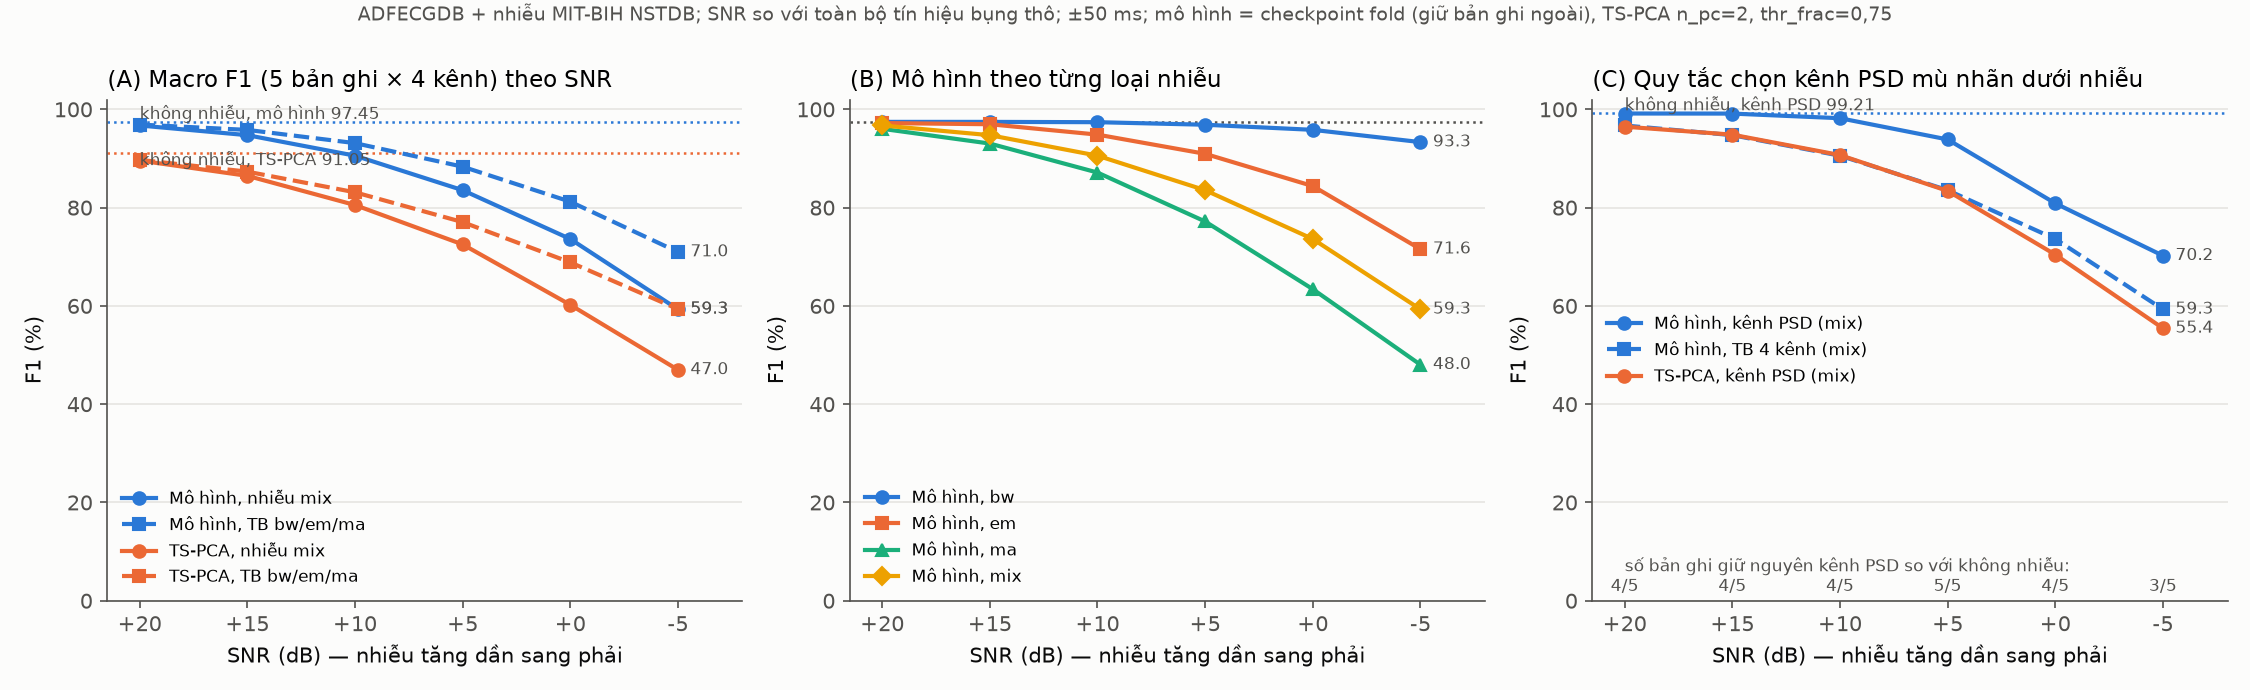
\includegraphics[width=\textwidth]{figs/fig14_snr.png}
\caption{(A) Macro F1 theo SNR, mô hình so với TS-PCA, nhiễu hỗn hợp và trung bình ba loại. (B) Mô hình
theo từng loại nhiễu: trôi nền gần như vô hại, nhiễu cơ hại nhất. (C) Quy tắc chọn kênh PSD mù nhãn dưới
nhiễu, kèm số bản ghi giữ nguyên kênh đã chọn so với khi không nhiễu.}
\label{fig:snr}
\end{figure}

\begin{table}[H]\centering\small
\caption{Macro F1 (5 bản ghi $\times$ 4 kênh) theo SNR. Không nhiễu: mô hình 97,45, TS-PCA 91,05.}
\label{tab:snr}
\begin{tabular}{@{}L{2.2cm} C{1.7cm} C{1.7cm} C{1.7cm} C{1.7cm} C{1.7cm} C{1.7cm}@{}}
\toprule
\textbf{Loại nhiễu} & \textbf{+20\,dB} & \textbf{+15} & \textbf{+10} & \textbf{+5} & \textbf{0} & \textbf{$-$5} \\
\midrule
\multicolumn{7}{@{}l}{\cellcolor{rowbg}\textbf{Mô hình}} \\
Trôi nền (bw) & 97,45 & 97,44 & 97,38 & 96,87 & 95,83 & 93,33 \\
Điện cực (em) & 97,21 & 96,97 & 94,86 & 90,95 & 84,38 & 71,55 \\
Nhiễu cơ (ma) & 96,04 & 93,03 & 87,13 & 77,18 & 63,41 & \xau{48,03} \\
Hỗn hợp (mix) & 96,71 & 94,74 & 90,57 & 83,55 & 73,62 & 59,31 \\
\multicolumn{7}{@{}l}{\cellcolor{rowbg}\textbf{TS-PCA}} \\
Trôi nền (bw) & 91,15 & 90,91 & 90,60 & 89,68 & 88,42 & 85,76 \\
Điện cực (em) & 90,56 & 89,17 & 84,96 & 79,50 & 69,81 & 56,79 \\
Nhiễu cơ (ma) & 87,44 & 81,89 & 73,80 & 61,98 & 48,34 & 35,50 \\
Hỗn hợp (mix) & 89,58 & 86,46 & 80,52 & 72,51 & 60,22 & 47,00 \\
\multicolumn{7}{@{}l}{\cellcolor{rowbg}\textbf{Chênh lệch mô hình $-$ TS-PCA, hỗn hợp}} \\
& $+7{,}13$ & $+8{,}28$ & $+10{,}04$ & $+11{,}04$ & \tot{$+13{,}40$} & $+12{,}31$ \\
\bottomrule
\end{tabular}
\end{table}

Bốn điều rút ra:

\begin{enumerate}[leftmargin=1.6em,itemsep=4pt]
\item \textbf{Trôi đường nền gần như vô hại.} Mô hình mất 4 điểm ở $-5$\,dB. Đây là tính chất của bộ lọc
10--60\,Hz: trôi nền nằm dưới 0,5\,Hz và bị loại trước khi vào mạng. Kết quả này \textit{không} nói lên
độ bền của mạng, mà nói lên front-end đúng.
\item \textbf{Nhiễu cơ là kẻ thù thật.} Phổ của nó trùng dải 10--60\,Hz nên bộ lọc không cản được. Mô hình
xuống dưới 90 ở khoảng $+10$\,dB và dưới 80 ở $+5$\,dB.
\item \textbf{Khoảng cách với cổ điển tăng khi nhiễu tăng}: từ $+7$ điểm khi sạch lên $+13$ điểm ở 0\,dB
hỗn hợp, $+15$ ở nhiễu cơ. Mạng không chỉ chính xác hơn mà còn \textit{gãy chậm hơn}.
\item \textbf{Quy tắc chọn kênh PSD ổn định đến 0\,dB} (4/5 hoặc 5/5 bản ghi giữ nguyên kênh), chỉ đổi
ở $-5$\,dB (3/5). F1 trên kênh PSD dưới nhiễu hỗn hợp: 99,21 khi sạch, 70,2 ở $-5$\,dB.
\end{enumerate}

Mã tại \texttt{pilot\_evidence/snr\_curve.py}; toàn bộ lưới (bản ghi $\times$ kênh $\times$ loại $\times$ SNR)
trong \texttt{snr\_curve.json}. Chạy 673 giây.
